\documentclass{article}
\usepackage[main, final]{neurips_2025}

\usepackage[utf8]{inputenc}
\usepackage[T1]{fontenc}
\usepackage{hyperref}
\usepackage{url}
\usepackage{booktabs}
\usepackage{amsfonts}
\usepackage{amsmath}
\usepackage{nicefrac}
\usepackage{microtype}
\usepackage{xcolor}
\usepackage{graphicx}
\usepackage{enumitem}
\usepackage{multirow}
\usepackage{tikz}
\usetikzlibrary{arrows.meta,positioning,fit,calc}

\makeatletter
\renewcommand{\@notice}{}
\makeatother

\title{Constraint-Contract Multi-Agent Repair for Travel Planning}

\author{
  Yuxuan Shu \\
  School of Intelligence Science and Technology, Nanjing University \\
  Nanjing, China \\
  \texttt{yuxuanshu@smail.nju.edu.cn}
}

\begin{document}

\maketitle

\begin{abstract}
Large language models can write plausible travel itineraries, but on TravelPlanner they often fail database-grounded hard constraints such as minimum-night rules, budget limits, room requirements, and transportation consistency. We study this failure mode under our local reproduction of the official TravelPlanner evaluation protocol and introduce \emph{Constraint-Contract Multi-Agent Repair} (CC-MAR), a verifier-mediated repair algorithm in which agents propose contract-level patches, a critic estimates cross-contract risk, and a mediator accepts only verifier-improving edits. On the 180-instance validation set, direct prompting reaches 20.00\% Final Pass Rate. Archived checklist and self-refinement artifacts score 20.00\% and 12.22\%, respectively, but provenance review reveals fallback and parsing failures that prevent interpreting them as clean independent strong baselines. CC-MAR improves Final Pass Rate to 35.00\%, and its ablations show small but mixed effects: removing the critic lowers performance to 33.89\%, removing the board lowers it to 34.44\%, but removing role specialization reaches 36.11\%. A separately engineered seeded verifier-repair pipeline reaches 46.67\%, and a narrower repair-heavy control reaches 48.89\%. These results indicate that explicit verification and local repair are the dominant sources of reliability; contract-mediated multi-agent repair provides a more controlled and inspectable protocol, but it does not outperform benchmark-specific deterministic repair in this setting.
\end{abstract}

\section{Introduction}
Travel planning is an attractive testbed for language agents because success depends on more than fluent text generation. A system must combine route construction, database-grounded entity selection, cost control, and user-specific hard constraints within a single itinerary \citep{xie2024travelplanner}. In TravelPlanner, failures such as picking an accommodation with an impossible minimum-night requirement or mixing incompatible transportation modes are fatal even when the itinerary is otherwise coherent.

Prior approaches in this repository expose the central difficulty. A direct-prompt baseline with \texttt{deepseek-v4-flash} reaches only 20.00\% Final Pass Rate under our reproduced protocol. A purely programmatic planner falls to 8.89\%, and a later LLM-assisted program planner reaches 12.22\%, which is still below direct prompting. These numbers matter because they show that simply adding more structure does not solve the benchmark. The bottleneck is not only plan generation; it is the absence of a reliable mechanism for detecting and repairing specific constraint violations after a candidate itinerary is written.

Our starting point is a simple observation: in TravelPlanner, many hard failures are externally checkable. Accommodation minimum-night violations, unsupported transportation choices, budget overruns, and several local constraints can be audited against the benchmark database without consulting the final scorer. This changes the problem from asking one model to implicitly track every constraint into a more controlled pipeline: produce candidate plans, expose their failures with a deterministic verifier, and revise only the failing fields or route segments.

We instantiate this idea in two systems. The first is a seeded verifier-repair pipeline that combines direct and program drafts with conservative local repair. The second, \emph{Constraint-Contract Multi-Agent Repair} (CC-MAR), is a verifier-mediated multi-agent algorithm: agents independently propose contract-specific patches, a critic reviews cross-contract risk, and a mediator accepts only patches that improve the deterministic verifier's violation vector.

This positioning is important for the paper's main claim. The strongest result is not produced by the most agentic system: a repair-heavy control reaches 48.89\%, the seeded role pipeline reaches 46.67\%, and CC-MAR reaches 35.00\%. The paper therefore does not argue that adding agent roles is automatically beneficial. Instead, CC-MAR tests a narrower claim: multi-agent repair becomes scientifically meaningful only when agents communicate through explicit constraint contracts and when promotion is governed by verifier-monotone acceptance.

Our contributions are:
\begin{itemize}[leftmargin=1.5em]
    \item We formulate TravelPlanner as a constrained generation problem in which hard feasibility can be partially externalized into deterministic verification.
    \item We introduce CC-MAR, a verifier-mediated multi-agent repair algorithm in which contract agents propose patch candidates and a mediator accepts only verifier-improving repairs.
    \item We package a reproducible local evaluation setup that preserves TravelPlanner scoring logic while redirecting validation data loading to local files in \texttt{database/validation.csv}.
    \item We compare direct prompting, stronger structured prompting, generic self-refinement, deterministic repair, CC-MAR, and communication/specialization ablations.
    \item We provide mechanism, cost, and failure analysis showing when contract-guided repair helps and which benchmark-grounded constraints remain difficult.
\end{itemize}

\section{Related Work}
\paragraph{LLM-based planning.}
Recent work has studied language models as planning agents that interleave reasoning and action \citep{yao2023react} or expand search over multiple thoughts \citep{yao2023treeofthoughts}. These methods show that decomposition can help difficult decision-making tasks, but they do not by themselves guarantee database-grounded constraint satisfaction. Our setting differs in that many failures are externally checkable, so verification is not a formatting choice but the main design variable.

\paragraph{Self-refinement and critique.}
Self-refinement methods use iterative feedback to improve model outputs \citep{madaan2023selfrefine,shinn2023reflexion}. This line of work motivates our multi-round design, but generic self-critique is often too weak for benchmark constraints that depend on a fixed entity database. In our system, critique is grounded by deterministic audit results, so the reviser receives explicit failure types instead of free-form advice.

\paragraph{Program-aided reasoning and verification.}
Program-aided LLM methods offload parts of reasoning to external code \citep{gao2022pal}, while decomposition-style prompting methods separate planning from execution \citep{wang2023planandsolve,wang2022selfconsistency}. Our work is closest in spirit to these approaches: instead of trusting a single forward pass, we use programmatic checks to expose failure modes that the model frequently misses. The difference is that we study which externalized failures matter most on a multi-constraint travel-planning benchmark with end-to-end constraint evaluation.

\paragraph{Benchmarking and LLM-based evaluation.}
TravelPlanner provides a realistic planning benchmark with structured reference information and constraint-aware evaluation \citep{xie2024travelplanner}. We use the benchmark scorer only for final reporting, not for per-sample selection. For internal judgment, we draw on the broader idea that LLM-based evaluation can be useful when paired with structured criteria \citep{liu2023geval}, but in our pipeline deterministic checks remain authoritative on all database-grounded constraints and LLM judgment is only a secondary signal.

\section{Problem Formulation}
Each TravelPlanner instance consists of a user request $q$, structured reference information $E$, and a set of benchmark constraints. The request specifies an origin city, destination region, trip length, number of travelers, budget, and optional local preferences such as cuisine or room type. The reference information provides candidate restaurants, attractions, accommodations, and transportation options extracted from the benchmark database.

The goal is to generate a day-level itinerary
\[
y = (d_1, d_2, \dots, d_T),
\]
where each day $d_t$ contains the current city, transportation, breakfast, attraction(s), lunch, dinner, and accommodation. Let $C_h$ denote hard constraints such as budget, valid entities, route closure, visiting-city count, transportation validity, minimum-night rules, and user-specified local constraints. Let $C_s$ denote softer quality criteria such as diversity or stylistic naturalness. A plan is \emph{feasible} if it satisfies all constraints in $C_h$.

Our objective is not to solve a global optimization problem exactly. Instead, we approximate
\[
\max_y U(y, q, E) \quad \text{subject to } y \text{ satisfies } C_h,
\]
where $U$ captures itinerary quality, while the benchmark scorer provides the final binary notion of success. In practice, the paper focuses on Final Pass Rate, the most stringent reproduced benchmark metric, and also reports commonsense and hard-constraint pass rates for diagnostic analysis.

\section{Method}
\subsection{Overview}
Figure~\ref{fig:pipeline} shows the seeded verifier-repair pipeline used in the earlier control experiments. The central design choice is to separate generation from verification. Rather than expecting one model call to track every benchmark constraint internally, we generate candidate itineraries, expose their failures through deterministic checks, and revise only the parts that the verifier marks as unsafe.

The final method, CC-MAR, makes this separation more explicit. It treats each checkable requirement as a \emph{constraint contract}. Contract agents independently propose patches for different failure classes, a critic estimates whether each patch may break another contract, and a deterministic mediator accepts only patches that improve the verifier's violation vector. This design gives the multi-agent system a concrete communication protocol and acceptance rule rather than a sequence of loosely connected prompts. We treat the particular role partition as an implementation choice and test it directly in ablations.

\begin{figure}[t]
    \centering
    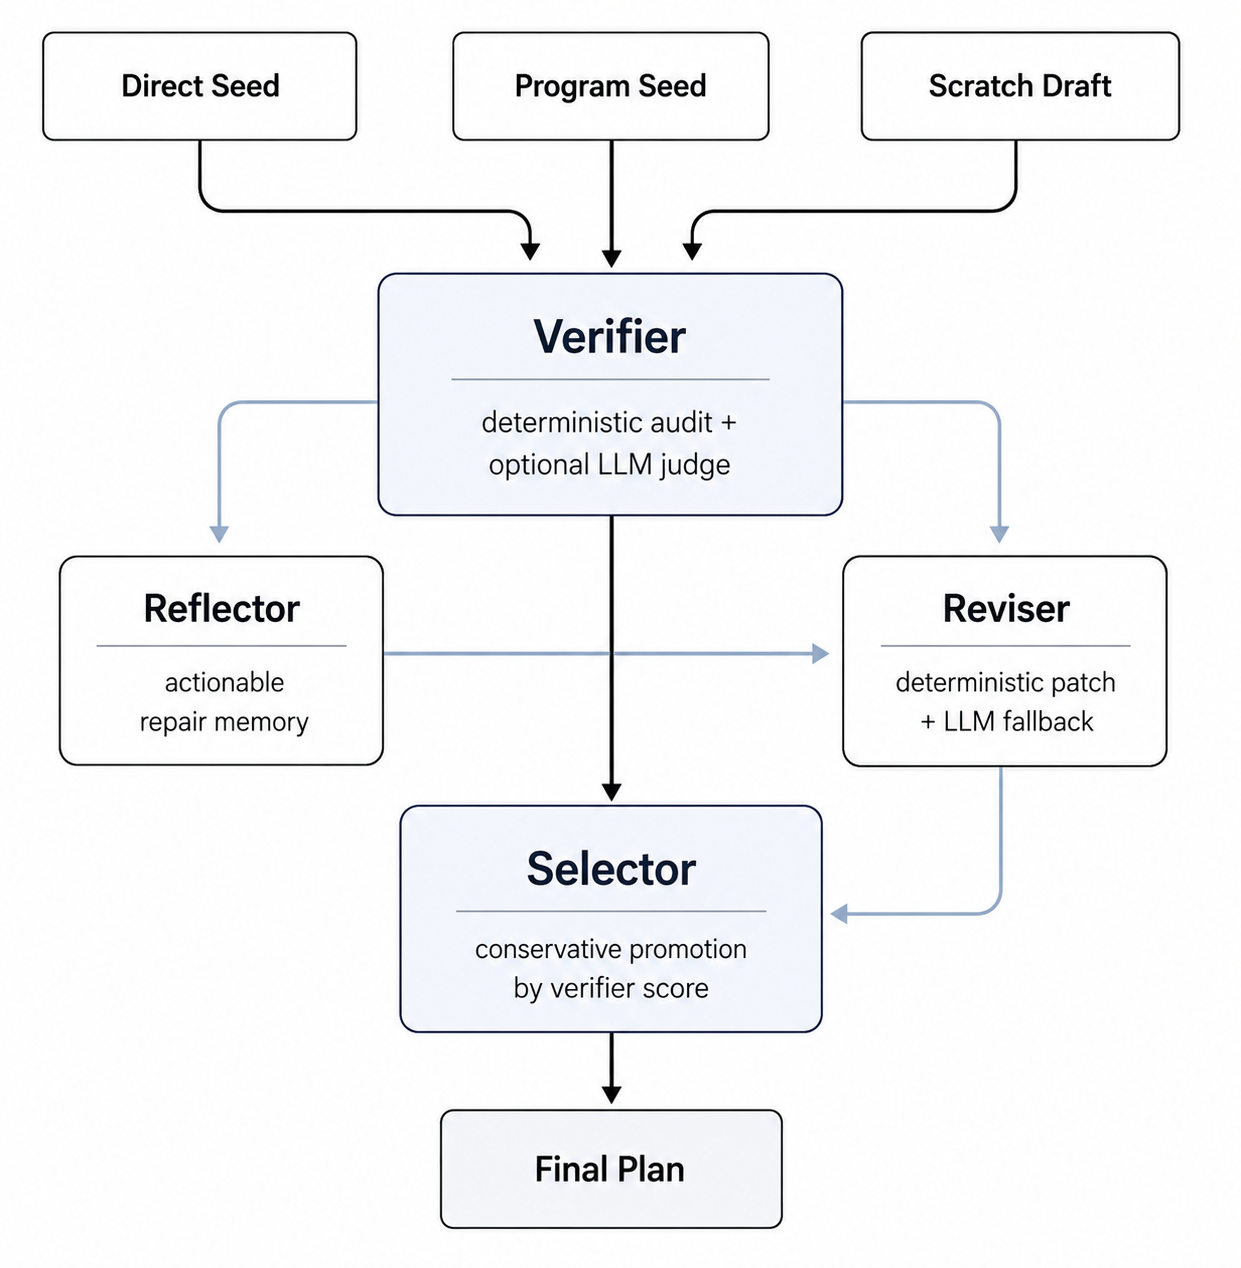
\includegraphics[width=0.84\linewidth, trim=25 25 25 25, clip]{assets/pipeline_figure.png}
    \caption{Overview of the planning pipeline. Multiple seed plans are audited by a verifier, repaired through reflection and revision, and conservatively promoted by a selector before producing the final plan. Dark arrows mark the main path from seeding to final selection, while lighter arrows show auxiliary repair flows.}
    \label{fig:pipeline}
\end{figure}

\subsection{Seeder Agent}
The seeder agent loads two heterogeneous drafts from local artifacts:
\begin{itemize}[leftmargin=1.5em]
    \item a direct-prompt itinerary from \texttt{outputs/validation};
    \item a program-generated itinerary from \texttt{outputs\_program\_v23\_best/validation}.
\end{itemize}
These drafts provide complementary strengths. The direct seed is usually stronger on overall completeness, while the program seed is often closer to database-supported transportation and entity choices.

When the seed pair is ambiguous or low-confidence, the planner agent additionally generates a scratch draft in structured JSON. In the final implementation, this scratch branch is activated adaptively: if the seed pair is already high-confidence under deterministic audit, the system skips scratch generation to save cost without changing the selection rule.

\subsection{Planner Agent}
The planner agent produces a structured itinerary rather than free-form prose. Its prompt explicitly asks for a route-first plan, exact day count, and concrete visited cities drawn from the reference candidates. This structured output reduces parse failures and makes downstream repair more local.

In the final system, the scratch planner is not claimed as the main driver of improvement. It acts as a diversity source on ambiguous cases. This distinction matters empirically: on many validation instances, the highest-leverage improvement comes from revising a flawed seed rather than inventing a fully new itinerary.

\subsection{Verifier Agent}
The verifier is the core reliability component. It combines deterministic benchmark-grounded checks with optional LLM judgments for tie-breaking and repair guidance. Deterministic checks are authoritative for:
\begin{itemize}[leftmargin=1.5em]
    \item route closure and visiting-city count;
    \item transportation validity and mode consistency;
    \item entity validity for restaurants, attractions, and accommodations;
    \item accommodation minimum-night rules;
    \item budget estimation;
    \item user local constraints such as room type, house rule, and cuisine.
\end{itemize}
The verifier assigns each candidate an audit score, a likely-pass flag, fatal issues, and warnings. Crucially, the final TravelPlanner evaluator is never used for per-sample selection.

\subsection{Reflector and Reviser Agents}
The reflector converts verifier outputs into actionable memory. For deterministically diagnosed errors such as minimum-night violations or budget overruns, the reflection can be generated directly from the audit signal. For more ambiguous cases, an LLM reflector summarizes concrete repairs instead of generic advice.

The reviser applies \emph{local repair}. It first attempts deterministic patches, with emphasis on the high-frequency failure modes observed in the repository:
\begin{itemize}[leftmargin=1.5em]
    \item replacing illegal accommodations with valid alternatives in the same city;
    \item inserting cuisine-compliant restaurants when required;
    \item reducing cost via cheaper valid meals or lodging.
\end{itemize}
If deterministic repair does not resolve the issue, the system falls back to an LLM reviser conditioned on the verifier evidence. Revised candidates are promoted only if they are conservatively better than the best seed under deterministic audit.

\subsection{Failure Handling and Reproducibility}
The full pipeline is resume-safe. All agent calls are cached, each instance writes an incremental debug file, and interrupted runs can continue with \texttt{RESUME=1}. This design is important because long API runs occasionally fail with transient network errors; the system is built to preserve partial progress rather than recomputing from scratch.

\subsection{Algorithmic Summary}
For each instance, the pipeline executes the following steps:
\begin{enumerate}[leftmargin=1.5em]
    \item Load the direct and program seed drafts, audit them deterministically, and rank them with a verifier-first score.
    \item Generate a scratch draft only when the seed pair is not already high-confidence.
    \item Apply deterministic verification to all round-1 candidates and call the optional LLM verifier only on selected candidates that are ambiguous, low-confidence, or newly generated.
    \item Choose repair targets from the verified pool, build reflection memory from explicit audit failures, and apply deterministic local repair before any LLM fallback.
    \item Re-verify revised candidates and promote them only when they are conservatively stronger than the best seed under deterministic audit.
    \item Let the selector break close ties among already promotable candidates, then emit the final plan and a per-instance debug record.
\end{enumerate}

\subsection{Constraint-Contract Multi-Agent Repair}
CC-MAR formalizes repair as contract-level patch arbitration. A contract $k \in K$ is a checkable predicate or partial predicate over a task $q$, environment $E$, and plan $y$. In TravelPlanner, contracts include route closure, city count, sandbox entity validity, transportation consistency, accommodation legality, budget, and user local constraints.

Given the deterministic verifier $V$, we summarize a plan by a violation vector
\[
\begin{aligned}
v(y) = (&\text{fatal},\ \text{invalid entities},\ \text{invalid transport},\
\text{min-night misses},\\
&\text{local misses},\ \text{budget miss},\ \text{warnings},\ -\text{score}).
\end{aligned}
\]
The mediator compares vectors lexicographically, where smaller is better. A patch $p$ is \emph{contract-dominating} if $v(p(y)) <_{\mathrm{lex}} v(y)$ and no protected hard contract changes from pass to fail.

Our default CC-MAR implementation uses five roles. The route agent proposes route and transportation repairs; the entity agent repairs sandbox and current-city violations; the lodging agent repairs minimum-night, room-rule, and room-type failures; the budget agent proposes cost and cuisine repairs; and the critic agent reviews proposed patches for cross-contract risk. Agents communicate only through a shared violation and patch board. The mediator is verifier-first: it re-audits each proposed patch and accepts at most one contract-dominating patch per round. Because role specialization is not assumed to be beneficial, we also evaluate no-specialization and single-agent variants.

\paragraph{Proposition.}
Under a deterministic verifier and finite patch budget, a CC-MAR run that accepts only contract-dominating patches produces a sequence of plans whose violation vectors monotonically improve under $V$ and terminates after finitely many accepted patches.

\paragraph{Proof sketch.}
Each accepted patch strictly decreases a finite lexicographic vector and is forbidden from regressing protected hard contracts. Because each round contains a finite number of proposed patches and the run has a finite round budget, the process cannot cycle. This guarantee is internal to the verifier; it does not guarantee reproduced benchmark validity or real-world travel feasibility.

\section{Experimental Setup}
\paragraph{Dataset.}
All experiments use the locally stored TravelPlanner validation split. The split contains 180 instances in \texttt{sole-planning} mode, balanced across difficulty levels and trip lengths.

\paragraph{Baselines.}
We compare against existing repository baselines, stronger prompt baselines, and repair controls:
\begin{itemize}[leftmargin=1.5em]
    \item \textbf{Direct Prompt}: a one-shot LLM itinerary generator;
    \item \textbf{Constraint-Checklist Direct}: a stronger structured direct prompt with explicit checklist constraints and JSON output;
    \item \textbf{Generic Self-Refine}: a prompt-only draft--critique--revise baseline without deterministic repair or verifier-based selection;
    \item \textbf{Program Planner v1}: a rule-based planner using extracted entities;
    \item \textbf{LLM-Assisted Program Planner}: the stored \texttt{program\_v23\_best} artifact;
    \item \textbf{Verifier-Guided Hybrid Selector}: a previous control that selects between direct and program drafts without structured multi-round repair.
\end{itemize}
We also report a \textbf{Verifier-Directed Repair Control}, the earlier seeded verifier-repair pipeline, and \textbf{CC-MAR}. For CC-MAR, we include ablations that remove the critic agent, remove the shared communication board, remove role specialization, or replace the specialist team with a single generic repair agent.

\paragraph{Model and decoding.}
All LLM-based components use \texttt{deepseek-v4-flash}. Structured direct generation uses temperature 0.1, generic self-refinement uses temperature 0.1 for drafting and 0.05 for revision, and CC-MAR agents use temperature 0.05 with a deterministic mediator. The earlier seeded pipeline uses two rounds, up to three candidates, and the default verifier-gated repair settings in \texttt{seeded\_multi\_agent\_planner.py}; CC-MAR uses three repair rounds unless otherwise stated.

\paragraph{Metrics.}
We report the TravelPlanner metrics produced by our local reproduction of the official evaluation protocol: Delivery Rate, Commonsense Constraint Micro/Macro Pass Rate, Hard Constraint Micro/Macro Pass Rate, and Final Pass Rate. Final Pass Rate is the primary metric.

\paragraph{Local evaluation pipeline.}
To make experiments reproducible in this environment, we preserve the original scoring logic while redirecting validation data loading to local files through \texttt{utils/local\_data.py} and \texttt{evaluation/run\_local\_eval.py}. We refer to this setup as \emph{our local reproduction of the official TravelPlanner evaluation protocol}. The final scorer is used only after a complete submission file is produced. It is never used for per-instance candidate selection, which relies only on internal verifier scores and deterministic repair checks. All headline numbers are artifact-level outcomes from single reproduced validation runs. The September 2026 appendix adds conditional paired intervals and separately labeled archived cross-model evidence; it does not convert the main table into repeated-run results. For internal auditing, a missing-accommodation marker on the final return day is treated as valid when the itinerary closes back at the origin, but all headline numbers in the paper are determined by the reproduced benchmark protocol rather than the internal audit alone.

\paragraph{Research questions.}
We organize the results around five questions: \textbf{RQ1} Does verifier-directed repair improve final validity over direct prompting and stronger prompt baselines? \textbf{RQ2} Does the gain come mainly from deterministic local repair or from multi-agent contract arbitration? \textbf{RQ3} Which CC-MAR components matter? \textbf{RQ4} How does the full pipeline use extra LLM budget in practice? \textbf{RQ5} Which benchmark constraints remain the main sources of failure?

\section{Results}
\begin{table}[t]
    \centering
    \caption{Main validation results under our local reproduction of the official TravelPlanner evaluation protocol. All entries are reproduced benchmark pass rates (\%, higher is better). The repair-heavy control remains strongest overall, while CC-MAR provides a contract-mediated multi-agent repair protocol that improves over prompt-only and generic self-refinement baselines.}
    \label{tab:main-results}
    \resizebox{\linewidth}{!}{\begin{tabular}{@{}lrrrrr@{}}
\toprule
Method & Final Pass (\%) $\uparrow$ & Common.\ Macro (\%) $\uparrow$ & Hard Macro (\%) $\uparrow$ & Common.\ Micro (\%) $\uparrow$ & Hard Micro (\%) $\uparrow$ \\
\midrule
\multicolumn{6}{@{}l}{\textit{Prompt-only and program baselines}} \\
Direct Prompt & 20.00 & 20.56 & 57.22 & 80.62 & 60.95 \\
Program Planner v1 & 8.89 & 21.11 & 16.67 & 71.67 & 24.05 \\
LLM-Assisted Program Planner & 12.22 & 18.33 & 42.78 & 82.15 & 35.48 \\
\midrule
\multicolumn{6}{@{}l}{\textit{Stronger prompting baselines}} \\
Constraint-Checklist Direct & 20.00 & 20.56 & 57.22 & 77.43 & 60.95 \\
Generic Self-Refine & 12.22 & 13.33 & 51.67 & 74.17 & 57.62 \\
\midrule
\multicolumn{6}{@{}l}{\textit{Verifier and repair controls}} \\
Verifier-Guided Hybrid Selector & 27.22 & 31.11 & 65.00 & 87.22 & 63.81 \\
Verifier-Directed Repair Control & \textbf{48.89} & \textbf{52.78} & \underline{68.89} & \textbf{90.90} & \underline{65.71} \\
\midrule
\multicolumn{6}{@{}l}{\textit{Seeded pipeline}} \\
Seeded Multi-Agent Planner & \underline{46.67} & \underline{49.44} & 67.22 & \underline{90.07} & 61.67 \\
\midrule
\multicolumn{6}{@{}l}{\textit{Contract multi-agent repair}} \\
CC-MAR & 35.00 & 38.33 & \textbf{72.22} & 88.26 & \textbf{71.19} \\
\bottomrule
\end{tabular}
}
\vspace{0.35em}

\begin{minipage}{\linewidth}
\footnotesize
\textit{Note:} Best values are bolded and second-best values are underlined. $^{\dagger}$ Historical baseline artifacts affected by fallback/parsing failures; see the provenance discussion in the updated appendix.
\end{minipage}
\end{table}

\begin{figure}[t]
    \centering
    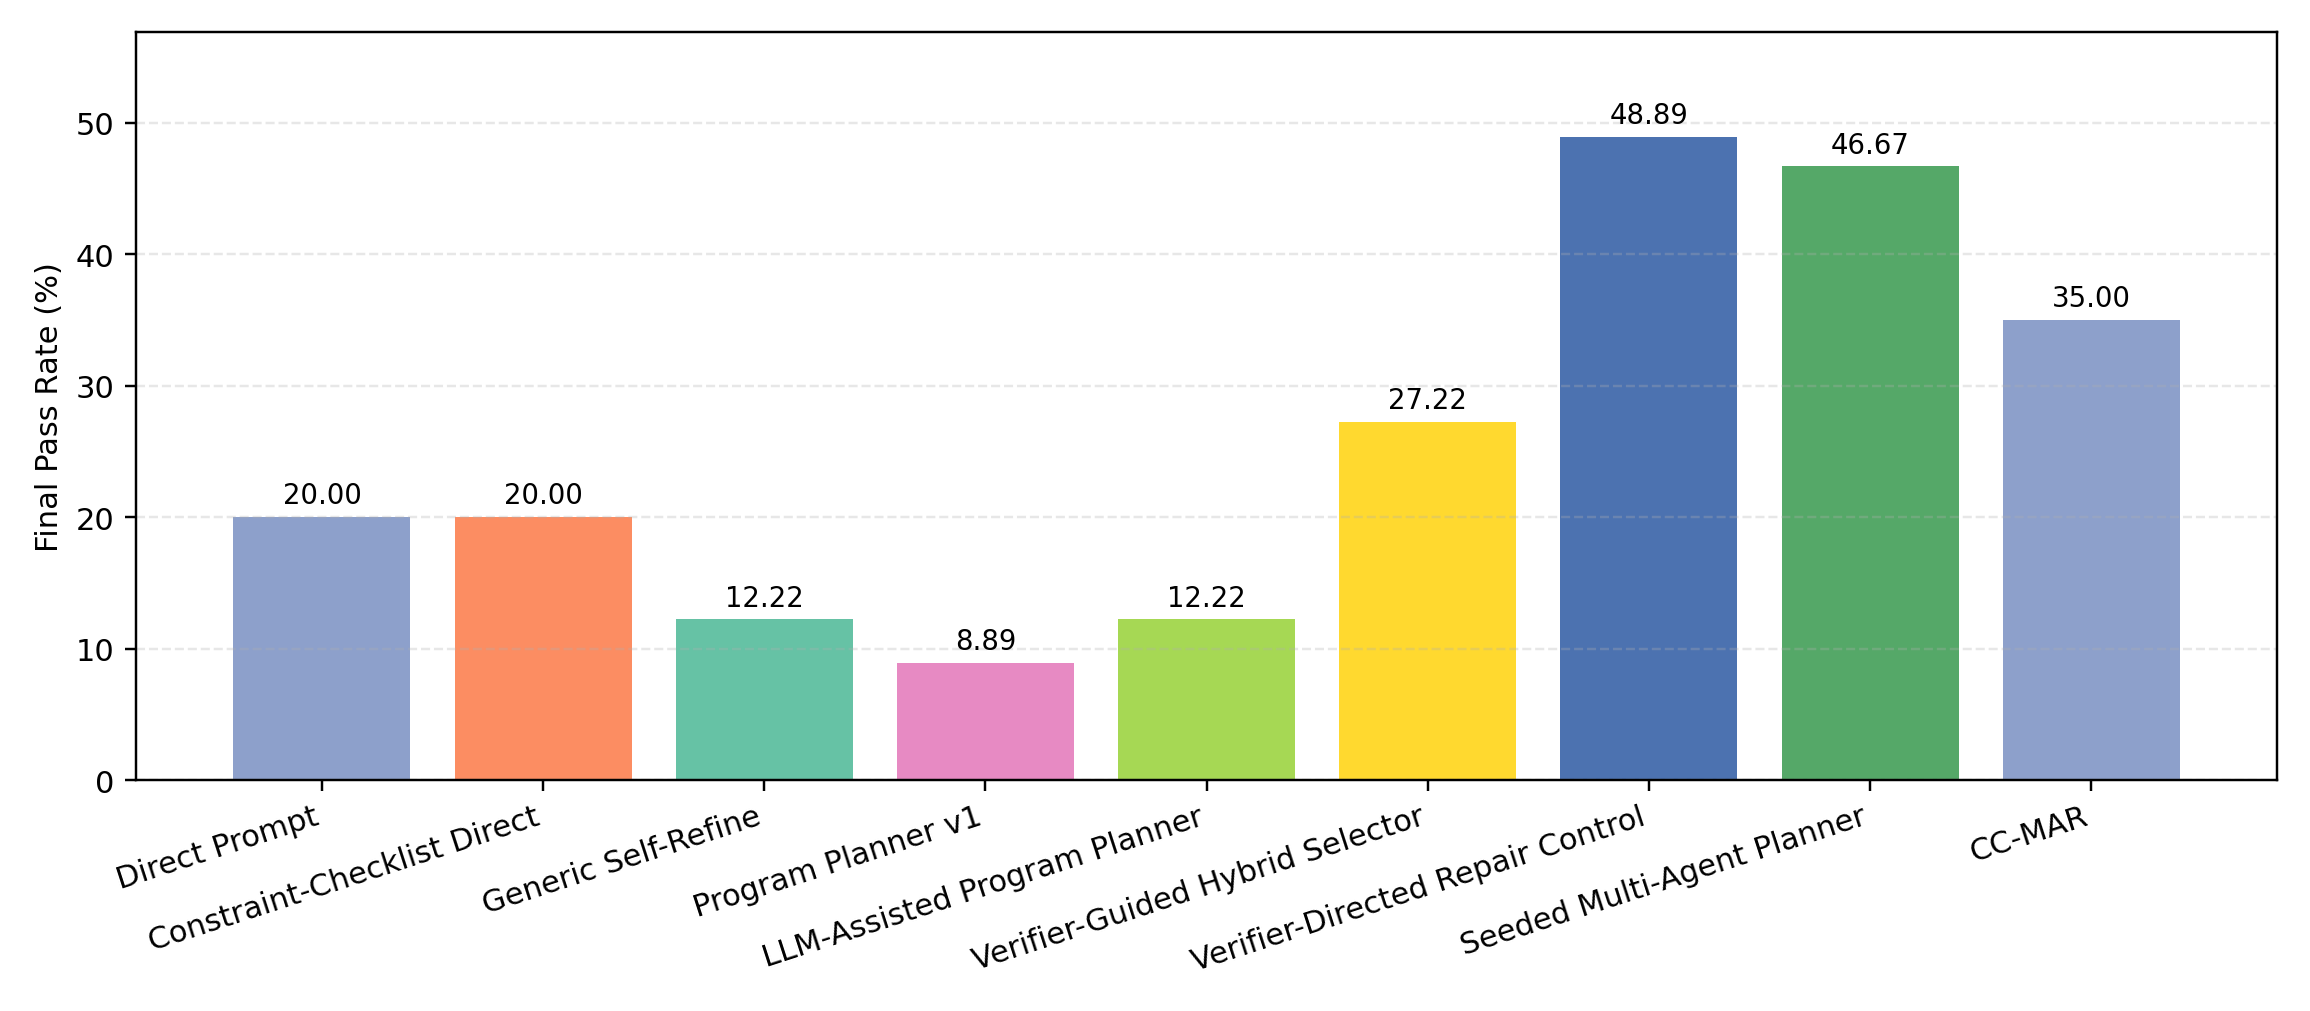
\includegraphics[width=0.92\linewidth]{assets/final_pass_rate.png}
    \caption{Final Pass Rate across reproduced baselines, controls, and repair methods. The large gap between prompt-only baselines and verifier-repair methods indicates that feasibility, not language fluency, is the main bottleneck on TravelPlanner.}
    \label{fig:final-pass}
\end{figure}

\paragraph{RQ1: Does verifier-directed repair improve final validity over direct prompting and earlier repository baselines?}
Yes. Table~\ref{tab:main-results} and Figure~\ref{fig:final-pass} show that validity improves materially only once the system can expose benchmark-grounded failures and repair them locally. Direct prompting reaches 20.00\% Final Pass Rate. The archived checklist artifact also scores 20.00\%, but all 180 checklist debug records indicate fallback (179 post hoc), so this does not establish the effect of a stronger prompt. The archived Self-Refine result is 12.22\%, with 92 failed revision parses and nine failed draft parses; its lower score cannot be attributed solely to the refinement algorithm. Verifier-based seed selection raises Final Pass Rate to 27.22\%, CC-MAR reaches 35.00\%, the full seeded pipeline reaches 46.67\%, and the repair-heavy control reaches 48.89\%.

The results separate two claims. First, verifier-directed local repair is the dominant empirical mechanism: the repair-heavy control improves Final Pass Rate by 28.89 points over direct prompting. Second, CC-MAR provides a more explicit multi-agent repair protocol, but its 35.00\% Final Pass Rate remains below the more benchmark-specific seeded repair systems. The central empirical conclusion is therefore not that more agents are inherently better; it is that hard-constraint exposure and conservative patch acceptance matter more than unconstrained generation or generic self-critique.

\begin{figure}[t]
    \centering
    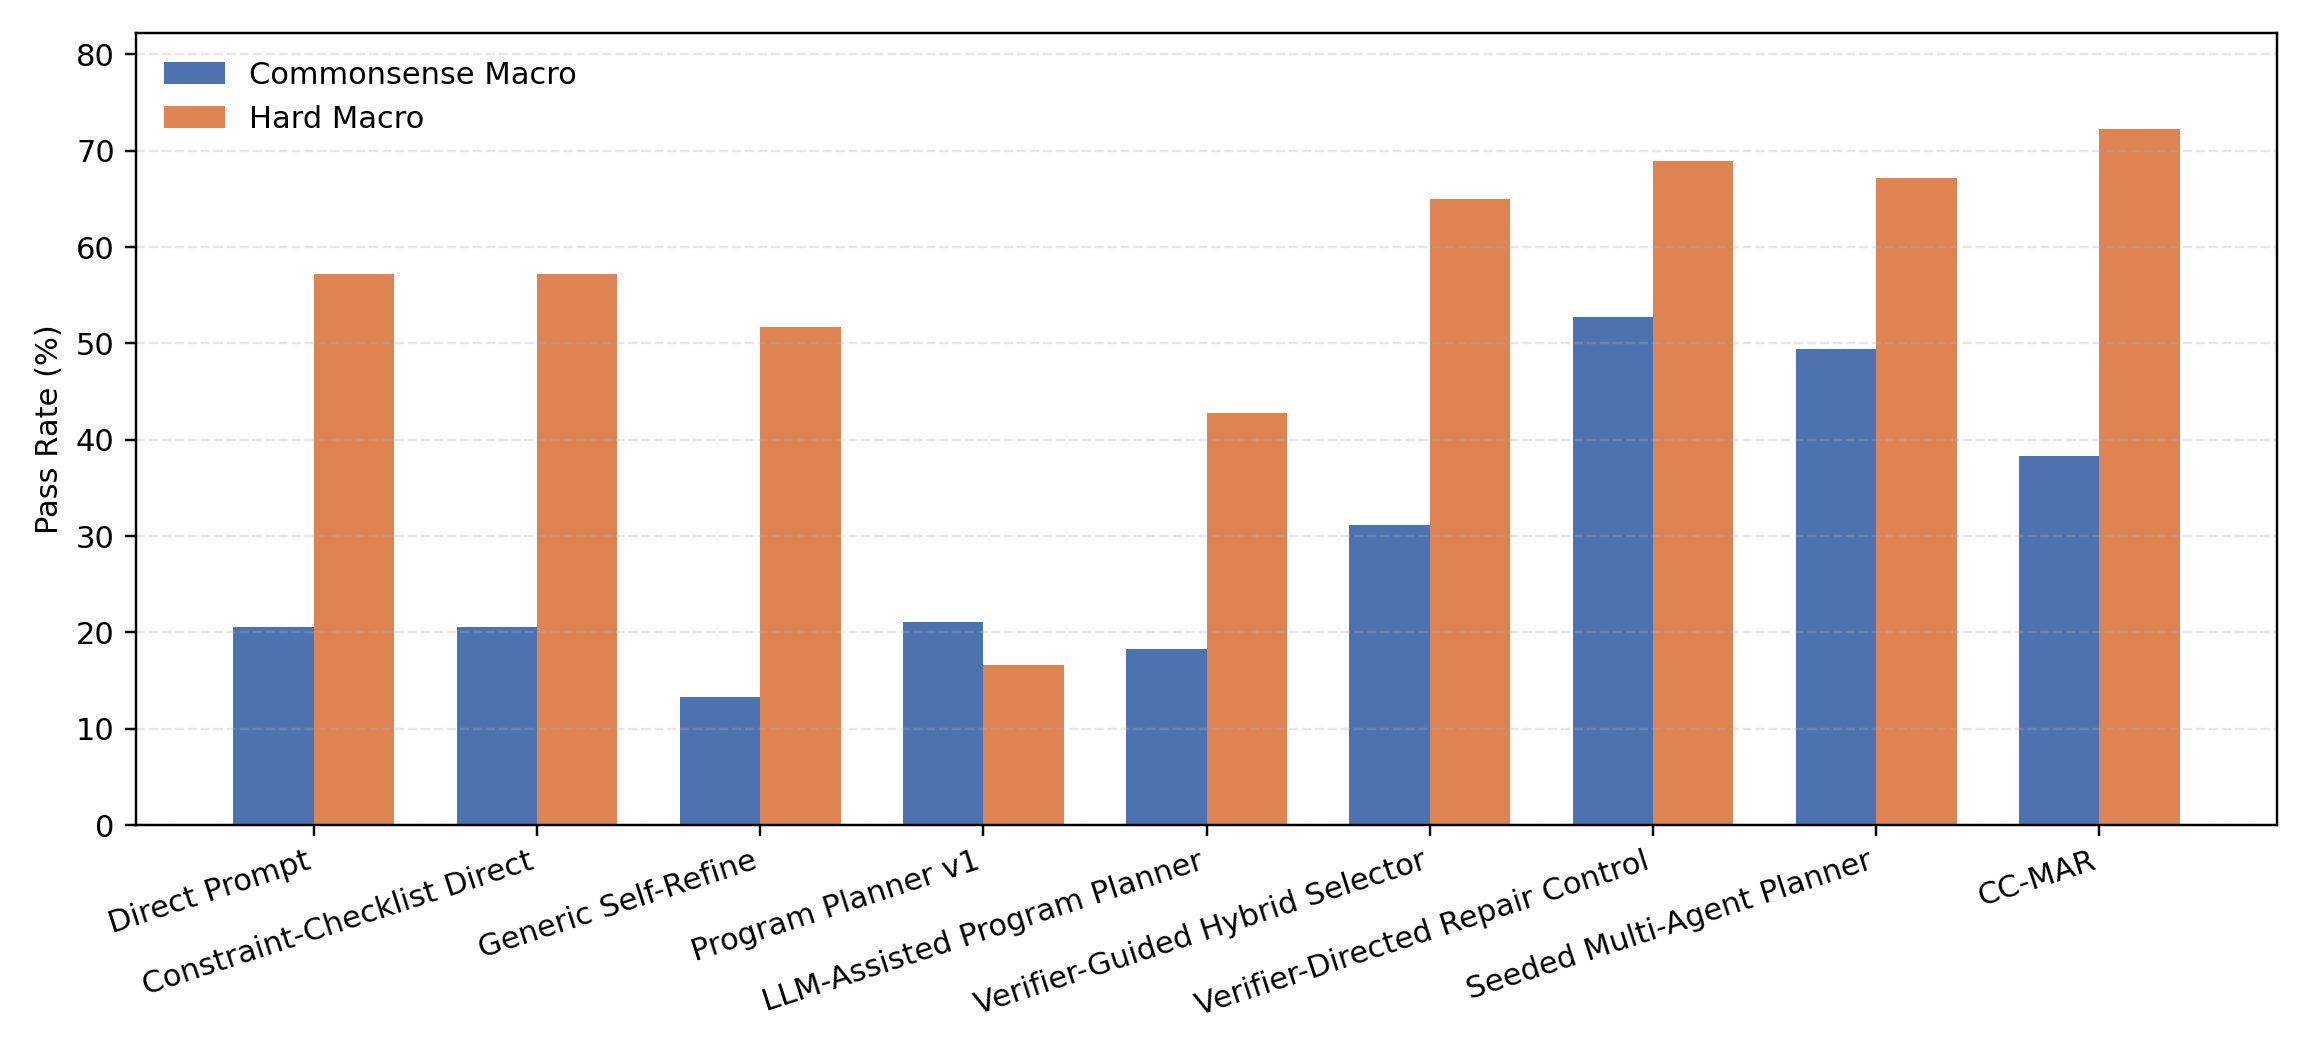
\includegraphics[width=0.92\linewidth]{assets/macro_breakdown.png}
    \caption{Macro-level commonsense and hard-constraint pass rates. Repair-based methods improve both axes simultaneously, suggesting that gains are not limited to one narrow subset of constraints.}
    \label{fig:macro-breakdown}
\end{figure}

\section{Analysis and Ablations}
\subsection{RQ2: Where does the gain come from?}
\begin{table}[t]
    \centering
    \caption{Progressive ablation of the main components. Verifier-based seed selection helps, but most of the gain comes from targeted repair. The full seeded loop remains much stronger than direct prompting even though the narrower repair control is slightly higher. All metrics are macro or final pass rates (\%, higher is better).}
    \label{tab:ablation}
    \resizebox{0.72\linewidth}{!}{\begin{tabular}{@{}lrrrr@{}}
\toprule
Variant & Final Pass (\%) $\uparrow$ & $\Delta$ Final vs.\ prev. & Common.\ Macro (\%) $\uparrow$ & Hard Macro (\%) $\uparrow$ \\
\midrule
Direct Prompt & 20.00 & -- & 20.56 & 57.22 \\
+ Verifier-Based Seed Selection & 27.22 & +7.22 & 31.11 & 65.00 \\
+ Deterministic Repair & 48.89 & +21.67 & 52.78 & 68.89 \\
+ Full Seeded Multi-Agent Loop & 46.67 & -2.22 & 49.44 & 67.22 \\
\bottomrule
\end{tabular}
}
\end{table}

Most of the gain comes from repair, not from additional agent freedom. Table~\ref{tab:ablation} shows that verifier-based seed selection improves Final Pass Rate from 20.00\% to 27.22\%, so heterogeneous drafts already contain useful complementary signal. The largest jump occurs when deterministic repair is added: Final Pass Rate rises by another 21.67 points to 48.89\%. The full seeded multi-agent loop then reaches 46.67\%, slightly below the repair-heavy control but still far above both direct prompting and seed selection alone.

This gap narrows the claim the paper can make. The results do not support the statement that freer multi-agent interaction is inherently stronger than a tighter repair policy on TravelPlanner. They support a more specific conclusion: seed diversity plus verifier-directed repair produces a much stronger planner than prompt-only generation, and the dominant mechanism is local correction guided by explicit failure exposure.

\subsection{RQ3: Which CC-MAR components matter?}
\begin{table}[t]
    \centering
    \caption{CC-MAR component ablations. The stored critic and shared-board contrasts show small numerical differences, but removing role specialization performs slightly better than the specialized-agent configuration. This negative result suggests that the current contract protocol is useful as controlled patch arbitration, while the particular role partition is not yet optimized.}
    \label{tab:cc-mar-ablation}
    \resizebox{0.78\linewidth}{!}{\begin{tabular}{@{}lrrrr@{}}
\toprule
Variant & Final Pass (\%) $\uparrow$ & Common.\ Macro (\%) $\uparrow$ & Hard Macro (\%) $\uparrow$ & Hard Micro (\%) $\uparrow$ \\
\midrule
CC-MAR & 35.00 & 38.33 & 72.22 & 71.19 \\
w/o Critic Agent & 33.89 & 37.22 & 71.67 & 69.52 \\
w/o Communication Board & 34.44 & 39.44 & 70.00 & 69.52 \\
w/o Role Specialization & 36.11 & 40.56 & 71.11 & 70.48 \\
Single Generic Repair Agent & 33.89 & 37.78 & 71.11 & 70.48 \\
\bottomrule
\end{tabular}
}
\end{table}

Table~\ref{tab:cc-mar-ablation} shows mixed evidence for the multi-agent components. Removing the critic lowers Final Pass Rate from 35.00\% to 33.89\%, and removing the shared board lowers it to 34.44\%, but paired confidence intervals include zero and these independently generated contrasts do not identify causal component effects. However, removing role specialization increases Final Pass Rate to 36.11\%, and a single generic repair agent reaches 33.89\%. These results do not support a strong claim that the chosen specialist decomposition is optimal. They support a narrower and more defensible claim: verifier-mediated patch arbitration improves over prompt-only baselines, while the best way to allocate repair responsibilities across agents remains open.

\subsection{Round-2 revision still matters inside the full pipeline}
On the diagnostic medium slice (instances 21--40), round-2 revision increases the best verifier score on 12 of 20 instances (60\%). The final selected plan is a revised candidate in 15 of 20 cases. This is important because it rules out a trivial explanation in which the system merely re-ranks pre-existing seeds.

The distribution of final choices on this slice is:
\begin{itemize}[leftmargin=1.5em]
    \item \texttt{program\_seed\_revised\_r2}: 14
    \item \texttt{program\_seed}: 2
    \item \texttt{direct\_seed}: 3
    \item \texttt{direct\_seed\_revised\_r2}: 1
\end{itemize}
This pattern suggests that the program seed provides a strong structural scaffold, while revision corrects the specific hard failures that prevent it from passing the reproduced benchmark protocol.

\subsection{RQ4: How does the full pipeline use extra LLM budget?}
\begin{table}[t]
    \centering
    \caption{Behavior and cost profile of the seeded multi-agent method on all 180 validation instances. Incremental LLM calls count scratch planning, first-round LLM verification, LLM reflection, and LLM revision beyond the two stored seed drafts. The profile shows that the system usually repairs or selects existing seeds rather than regenerating plans from scratch.}
    \label{tab:agent-profile}
    \resizebox{0.6\linewidth}{!}{\begin{tabular}{@{}lcc@{}}
\toprule
Statistic & Count / 180 & Share / Value \\
\midrule
\multicolumn{3}{@{}l}{\textit{Selection behavior}} \\
Final revised candidate selected & 101 & 56.1\% \\
Original seed selected & 79 & 43.9\% \\
\midrule
\multicolumn{3}{@{}l}{\textit{Adaptive generation}} \\
Scratch planner generated & 68 & 37.8\% \\
Scratch planner skipped & 112 & 62.2\% \\
\midrule
\multicolumn{3}{@{}l}{\textit{Reflection mode}} \\
Deterministic reflection & 133 & 73.9\% \\
LLM reflection & 47 & 26.1\% \\
\midrule
\multicolumn{3}{@{}l}{\textit{LLM budget}} \\
Average incremental LLM calls / instance & \multicolumn{2}{c@{}}{2.21} \\
Maximum incremental LLM calls & \multicolumn{2}{c@{}}{6} \\
\bottomrule
\end{tabular}
}
\end{table}

\begin{figure}[t]
    \centering
    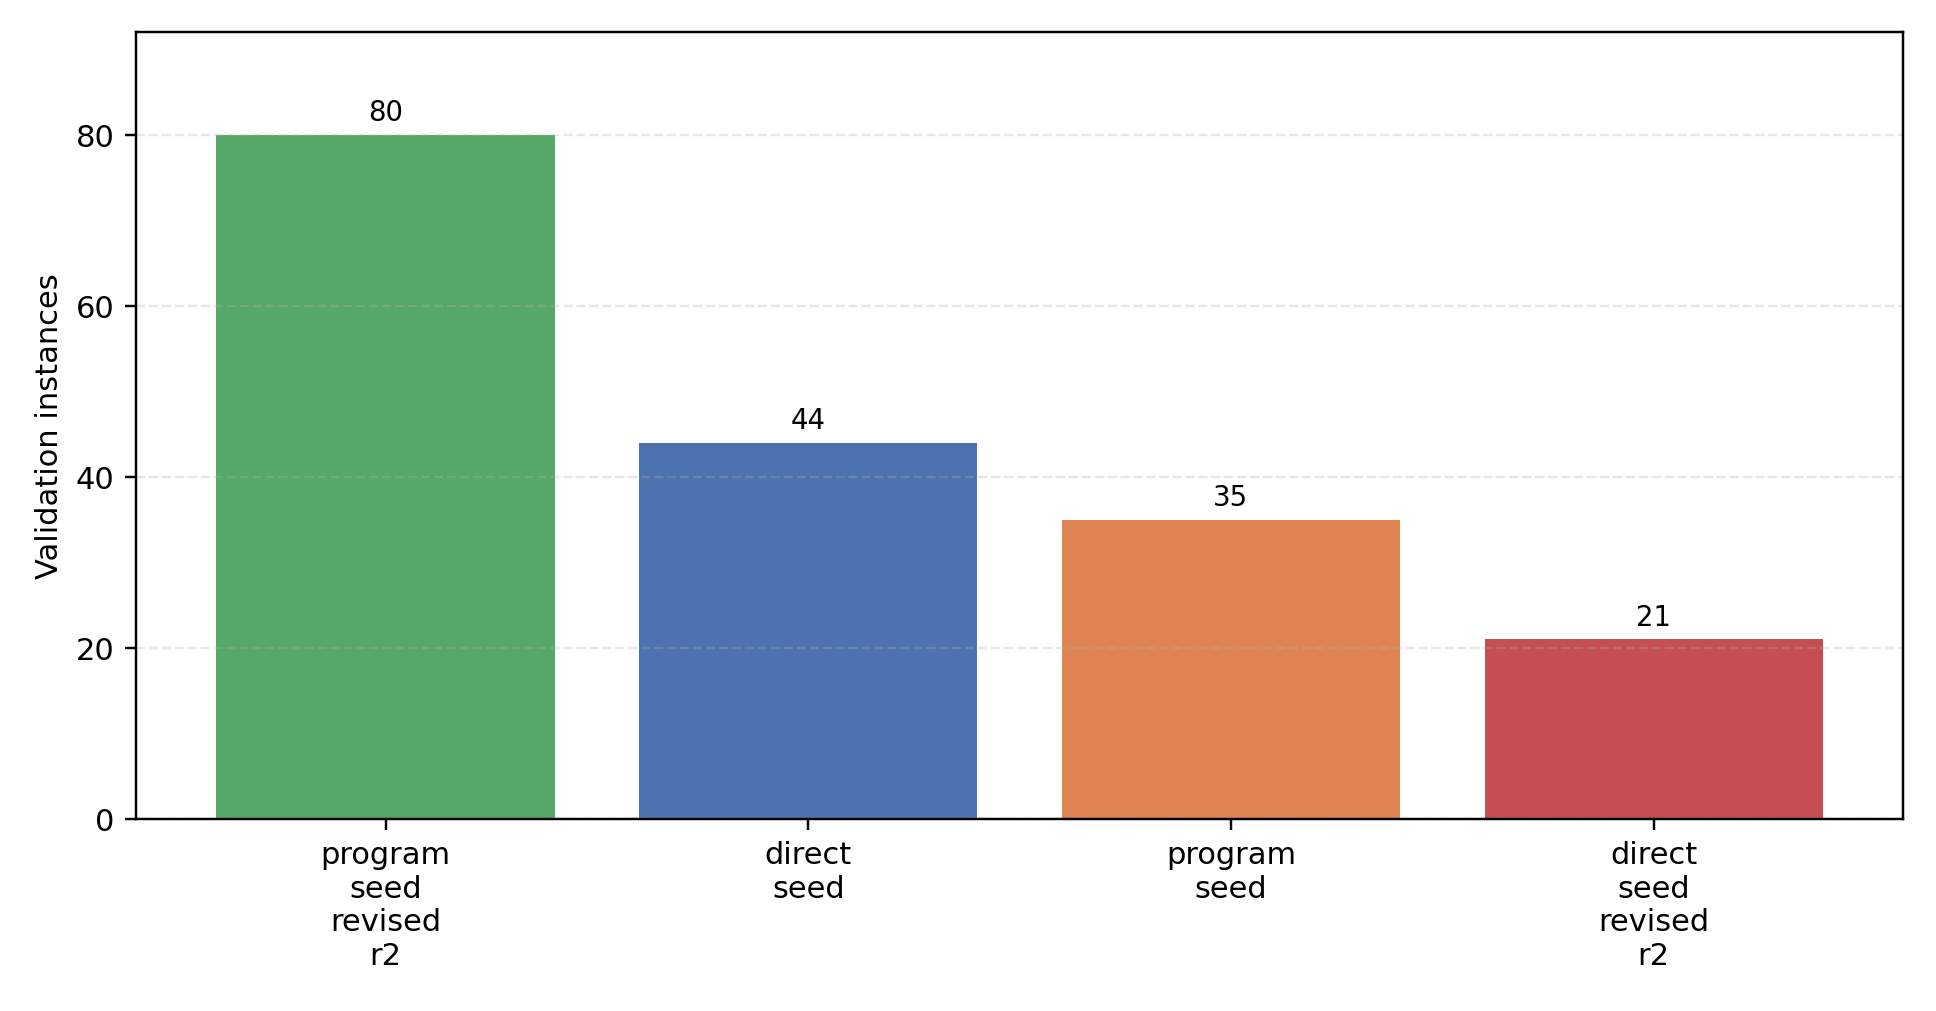
\includegraphics[width=0.84\linewidth]{assets/selection_distribution.png}
    \caption{Distribution of final selections for the seeded multi-agent planner. Most wins come from repairing the program seed, while direct and program seeds still survive unchanged on a substantial minority of instances.}
    \label{fig:selection-distribution}
\end{figure}

Table~\ref{tab:agent-profile} and Figure~\ref{fig:selection-distribution} show that the method behaves conservatively rather than rewriting everything. A revised candidate is selected in 101 of 180 instances, while an original seed remains best in 79 cases. The most common final choice is \texttt{program\_seed\_revised\_r2} (80 instances), followed by \texttt{direct\_seed} (44), \texttt{program\_seed} (35), and \texttt{direct\_seed\_revised\_r2} (21). The scratch planner is invoked on only 68 instances and skipped on 112 high-confidence seed pairs, which keeps the average incremental LLM budget at 2.21 calls per instance. This supports the intended design: use seed diversity and explicit repair first, and reserve fresh generation for ambiguous cases.

\subsection{What the Reviser Actually Fixes}
The strongest internal evidence comes from the repair logs. Under deterministic audit, successful direct/program repairs are dominated by accommodation substitution. Across the full validation set, deterministic repair produces 57 additional audit-clean plans beyond the original seed union, and 82 successful repairs include an accommodation patch. Budget-reduction patches appear much less frequently, and cuisine-driven patches are rare.

This asymmetry is informative rather than incidental. It indicates that the current benchmark state is dominated by a narrow class of high-impact hard failures: seed plans often choose otherwise plausible accommodations that violate minimum-night rules or local lodging constraints. These failures are easy to miss in end-to-end prompting but easy to repair once surfaced explicitly.

\subsection{RQ5: Which constraints remain difficult?}
\begin{table}[t]
    \centering
    \caption{Remaining failure taxonomy for the seeded multi-agent method under our reproduced evaluation protocol. Counts aggregate criterion-level false checks from the benchmark detailed scores, so a single plan may contribute to multiple rows.}
    \label{tab:error-taxonomy}
    \resizebox{0.72\linewidth}{!}{\begin{tabular}{@{}lrr@{}}
\toprule
Failure category & False checks & Share of all false checks (\%) \\
\midrule
Diverse Restaurants & 36 & 22.64 \\
Non-conf. Transportation & 34 & 21.38 \\
Complete Information & 34 & 21.38 \\
Minimum Nights Stay & 25 & 15.72 \\
Within Sandbox & 10 & 6.29 \\
Room Type & 6 & 3.77 \\
Room Rule & 5 & 3.14 \\
Budget & 4 & 2.52 \\
\bottomrule
\end{tabular}
}
\end{table}

Table~\ref{tab:error-taxonomy} shows that the remaining errors are concentrated rather than diffuse. The most common false checks involve restaurant diversity, transportation consistency, complete-information checks, and minimum-night constraints. This pattern is consistent with the benchmark's structure: once budget and room-rule violations are repaired, the hardest residual cases are those that require coordinated day-level coverage across multiple fields rather than a single local substitution.

\subsection{Breakdown by Trip Length and Difficulty}
\begin{table}[t]
    \centering
    \caption{Final Pass Rate by difficulty level (\%, higher is better). Repair-based methods remain stronger than direct prompting across all difficulty groups, with the largest gains on easy and medium instances.}
    \label{tab:difficulty-breakdown}
    \resizebox{0.72\linewidth}{!}{\begin{tabular}{@{}lrrr@{}}
\toprule
Method & Easy (\%) $\uparrow$ & Medium (\%) $\uparrow$ & Hard (\%) $\uparrow$ \\
\midrule
Direct Prompt & 26.67 & 11.67 & 21.67 \\
Constraint-Checklist Direct & 26.67 & 11.67 & 21.67 \\
Generic Self-Refine & 20.00 & 1.67 & 15.00 \\
Program Planner v1 & 15.00 & 10.00 & 1.67 \\
LLM-Assisted Program Planner & 18.33 & 15.00 & 3.33 \\
Verifier-Guided Hybrid Selector & 35.00 & 23.33 & 23.33 \\
Verifier-Directed Repair Control & 78.33 & 40.00 & 28.33 \\
Seeded Multi-Agent Planner & 76.67 & 41.67 & 21.67 \\
CC-MAR & 48.33 & 28.33 & 28.33 \\
\bottomrule
\end{tabular}
}
\end{table}

\begin{table}[t]
    \centering
    \caption{Final Pass Rate by trip length (\%, higher is better). Long-horizon itineraries remain harder, but repair-based methods reduce the gap substantially on 5-day and 7-day trips.}
    \label{tab:days-breakdown}
    \resizebox{0.72\linewidth}{!}{\begin{tabular}{@{}lrrr@{}}
\toprule
Method & 3 days (\%) $\uparrow$ & 5 days (\%) $\uparrow$ & 7 days (\%) $\uparrow$ \\
\midrule
Direct Prompt & 40.00 & 13.33 & 6.67 \\
Constraint-Checklist Direct & 40.00 & 13.33 & 6.67 \\
Generic Self-Refine & 21.67 & 10.00 & 5.00 \\
Program Planner v1 & 26.67 & 0.00 & 0.00 \\
LLM-Assisted Program Planner & 28.33 & 5.00 & 3.33 \\
Verifier-Guided Hybrid Selector & 53.33 & 18.33 & 10.00 \\
Verifier-Directed Repair Control & 61.67 & 45.00 & 40.00 \\
Seeded Multi-Agent Planner & 61.67 & 40.00 & 38.33 \\
CC-MAR & 55.00 & 30.00 & 20.00 \\
\bottomrule
\end{tabular}
}
\end{table}

\begin{figure}[t]
    \centering
    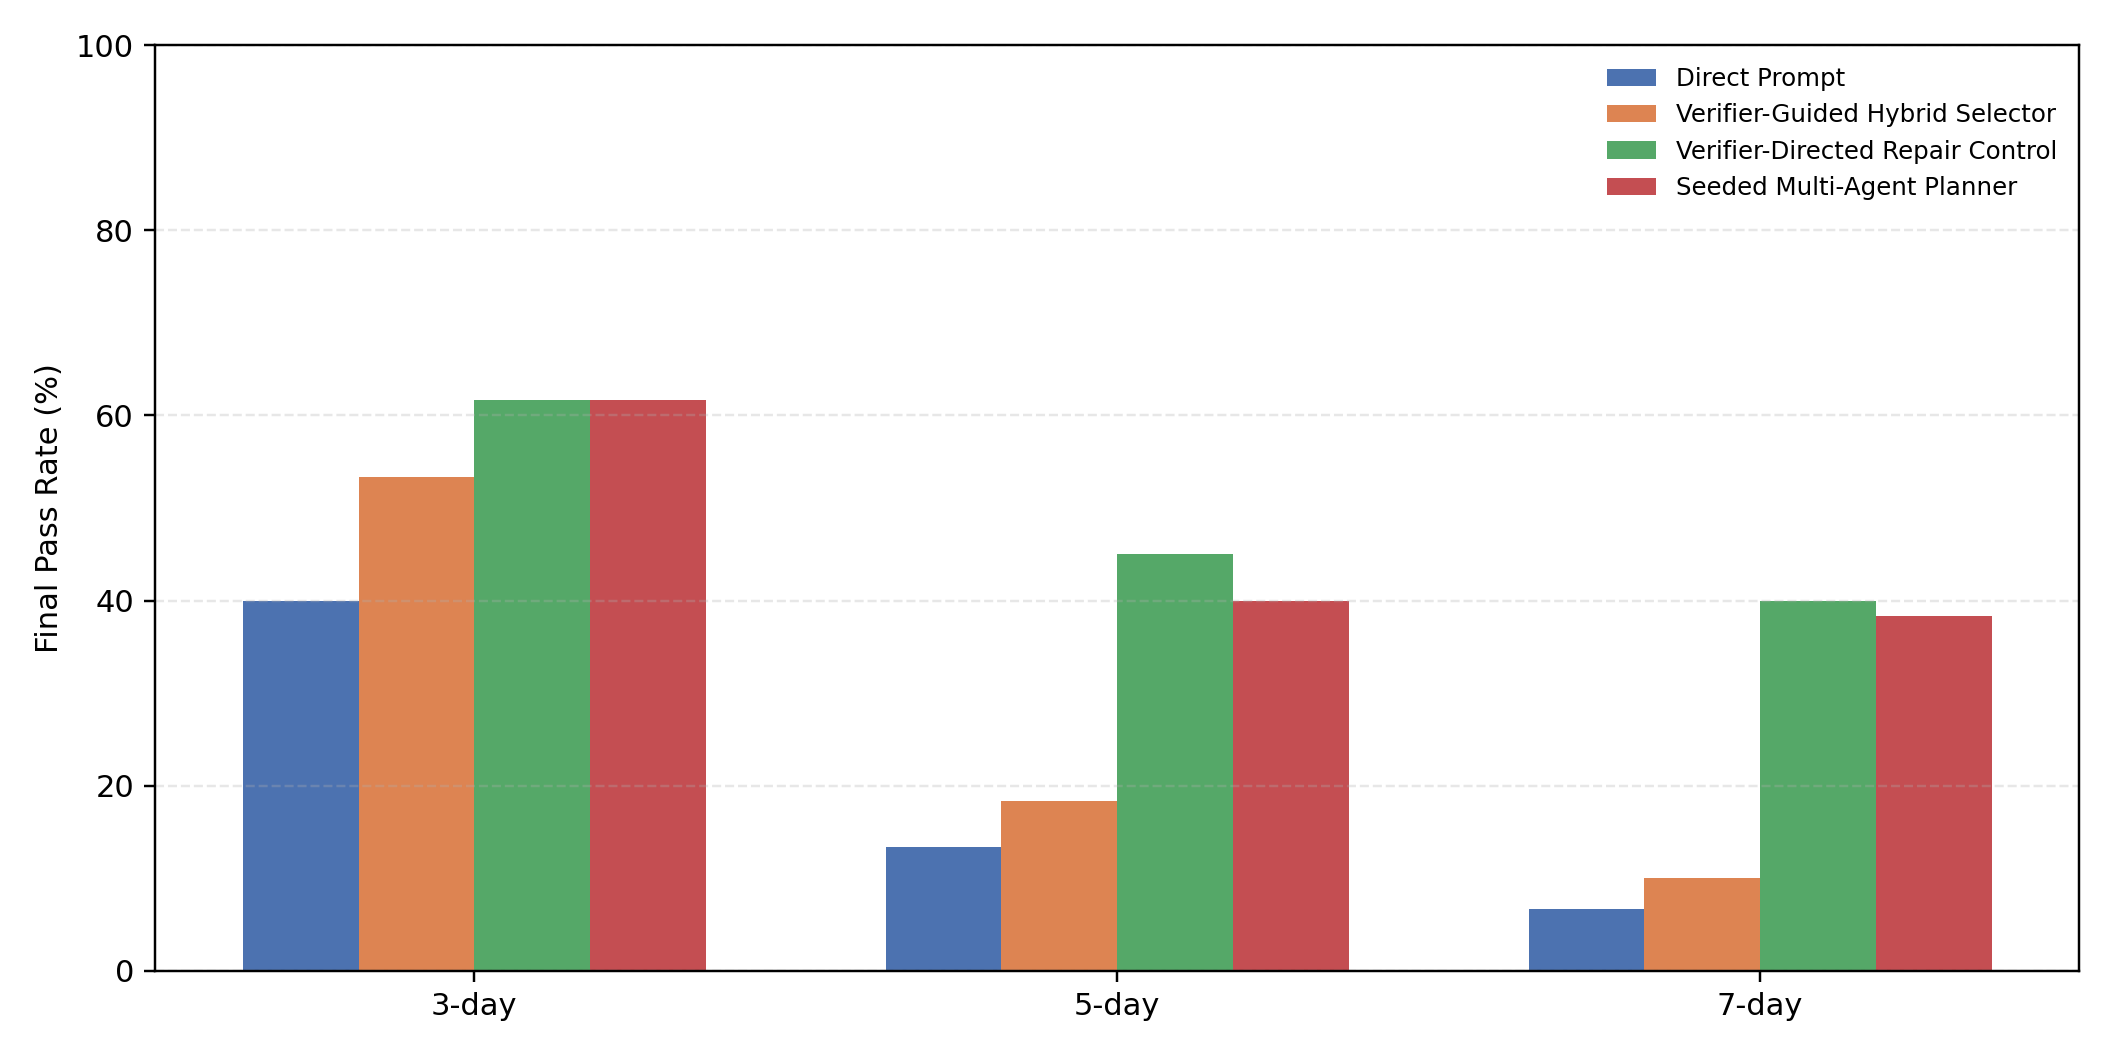
\includegraphics[width=0.92\linewidth]{assets/days_breakdown.png}
    \caption{Final Pass Rate by trip length for representative methods. Repair-based methods are especially valuable on 5-day and 7-day instances, where route continuity and accommodation legality interact more often.}
    \label{fig:days-breakdown}
\end{figure}

We further break down final-pass performance by difficulty and trip length in Tables~\ref{tab:difficulty-breakdown} and~\ref{tab:days-breakdown}. The broad pattern is that repair-based methods remain stronger across all groups. For the full seeded multi-agent method, the improvement over direct prompting is especially large on 5-day trips (40.00\% vs.\ 13.33\%) and 7-day trips (38.33\% vs.\ 6.67\%), while the repair-heavy control remains the strongest method on the hardest long-horizon settings.

\subsection{Case Studies}
Table~\ref{tab:case-studies} compresses three representative trajectories into a common format. The first two are successful because the pipeline preserves a strong route scaffold and patches a small number of high-impact fields. The third remains a failure because transportation legality is less local than accommodation replacement and can still break after otherwise sensible edits.

\begin{table}[t]
    \centering
    \caption{Representative repair trajectories. Successful cases usually preserve an existing scaffold and repair a small number of benchmark-critical fields, while the remaining failures involve less local transportation constraints.}
    \label{tab:case-studies}
    \resizebox{\linewidth}{!}{\begin{tabular}{@{}p{0.11\linewidth}p{0.27\linewidth}p{0.28\linewidth}p{0.24\linewidth}@{}}
\toprule
Case & Seed failure & Repair action & Outcome \\
\midrule
21 & Program seed uses an Orlando accommodation with a 30-night minimum stay. & Replace the lodging with a valid short-stay option and slightly reduce meal cost. & Converts a one-fatal plan into a likely-pass candidate under reproduced evaluation. \\
28 & Direct seed is incomplete and the program seed contains an invalid Norfolk accommodation. & Preserve the stronger route scaffold and patch the lodging locally. & Produces a complete five-day plan with verifier score 100 on the diagnostic run. \\
32 & Revised candidate still introduces an invalid flight despite otherwise plausible daily structure. & Attempt local transportation repair, then fall back to the LLM reviser when deterministic patching is insufficient. & Remains a benchmark failure, illustrating brittle route repair when the valid transport space is sparse. \\
\bottomrule
\end{tabular}
}
\end{table}

\section{Limitations}
The paper has several limitations.

First, the strongest full-validation result comes from a repair-heavy control (48.89\%) rather than from either the seeded role pipeline (46.67\%) or CC-MAR (35.00\%). This narrows the interpretation of our contribution: the main gain comes from explicit verifier-guided correction, while contract-mediated multi-agent repair adds a cleaner arbitration protocol and better diagnostics but not the absolute best score.

Second, the deterministic verifier and local repair rules are benchmark-specific. Although the checks are transparent and reproducible, they are written against the TravelPlanner database schema and cannot be assumed to transfer unchanged to other planning environments.

Third, the internal audit and the reproduced benchmark scorer are related but not identical. We avoid using the final scorer for per-sample selection, but this also means that some high-audit candidates still fail the reproduced benchmark metric. The paper therefore distinguishes internal audit analysis from final benchmark results whenever the two are compared.

Fourth, the CC-MAR ablations show that the current role specialization is not reliably beneficial: the no-specialization variant reaches 36.11\%, slightly above the specialized CC-MAR configuration. This does not invalidate verifier-mediated patch arbitration, but it does mean that the role design should be treated as an implementation choice rather than a settled algorithmic optimum.

Fifth, the main validation comparison remains single-run and the archived stronger-baseline artifacts have documented fallback/parsing limitations. The updated appendix reports three archived Qwen runs under proxy test evaluation, with incomplete request provenance; new controlled cross-model replications remain pending valid provider credentials. We therefore position the paper as a benchmark-grounded study of one reproduced setting rather than a broad claim of model-agnostic superiority.

Sixth, API-based experiments remain sensitive to runtime and networking noise. The system is resume-safe, but cost and wall-clock latency are still higher than single-pass prompting, and the scratch branch has not been isolated as an independent source of uplift beyond its role as an adaptive diversity mechanism.

\section{Ethics and Societal Impact}
This work studies benchmarked travel planning rather than deployment to real users. Even so, constraint-violating travel plans can be misleading or unsafe if used without verification. A language model may recommend infeasible transportation, illegal lodging arrangements, or budget-breaking itineraries. Our method reduces some of these risks by externalizing checkable constraints, but it does not eliminate the possibility of unsafe recommendations.

The benchmark itself is static and database-bounded. It does not model real-time availability, safety advisories, accessibility needs, or social bias in recommendations. As a result, a plan that passes benchmark constraints should not be interpreted as real-world travel advice. The main ethical value of this work is methodological: it shows how to make LLM planning more auditable in settings where external constraints are known.

\section{Conclusion}
This paper studies TravelPlanner through the lens of constraint exposure and local repair. Under our local reproduction of the official TravelPlanner evaluation protocol, CC-MAR improves Final Pass Rate from 20.00\% direct prompting to 35.00\%, while the full seeded verifier-repair pipeline reaches 46.67\% and the stronger repair-heavy control reaches 48.89\%. The clearest scientific conclusion is therefore not that multi-agent freedom is universally best, but that verifier-directed local repair is the dominant mechanism behind reliable benchmark performance in this setting.

CC-MAR remains useful because it turns multi-agent repair into an auditable protocol: agents propose patches, a critic records cross-contract risk, and a mediator accepts only verifier-improving edits. The fact that a no-specialization ablation slightly outperforms the specialized version is also informative: future progress may depend less on adding more named roles and more on tighter interfaces between generation, verification, arbitration, and local correction.

\bibliographystyle{plainnat}
\bibliography{references}

\appendix

\section{Implementation and Reproducibility Details}
\subsection{Algorithmic and modeling scope}
\paragraph{Role-specialized multi-agent scope.}
The paper uses ``multi-agent'' in an operational sense: agents have distinct prompts, explicit input/output contracts, a shared board, critic review, and mediator-controlled promotion, but they share the same base model. We do not claim decentralized learning, strategic negotiation, or emergent cooperation.

\paragraph{Current public artifact.}
The September 2026 repository update includes 13 frozen validation submissions,
per-instance Final Pass outcomes, expected metrics, and SHA-256 hashes in
\path{results/frozen}. Task queries, the benchmark database, credentials and raw
provider traces are excluded. All 13 metric rows and all stored Final Pass labels
were re-scored without discrepancies. The deterministic repair reconstruction
matches all 180 historical plans exactly and reproduces 88/180 Final Pass.

\paragraph{Data and offline reproduction.}
Install \path{requirements-research.txt}, obtain the official TravelPlanner database,
and set \texttt{TP\_DATABASE\_DIR} if it is outside the project. From the repository root:
\begin{verbatim}
python -m scripts.verify_frozen
python -m scripts.prepare_data
python -m scripts.reproduce --output runs/reproduced_repair.jsonl
python -m scripts.evaluate_submission_subset --set-type validation \
  --input runs/reproduced_repair.jsonl --output runs/metrics.json
python -m scripts.replay_frozen
python -m scripts.analyze_evidence
python -m scripts.build_public_artifacts
\end{verbatim}
The first command requires no database or model access. Reconstruction explicitly
uses \texttt{legacy-v1}. The reproduction and experiment guides document optional
seed paths, the recovered Program generator, and new model runs.

\paragraph{Evaluation and checkpoints.}
Full and subset evaluation share \path{evaluation/protocol.py}; sample IDs are
validated and aligned, and unevaluated applicable constraints remain in Micro
metric denominators. The full entry point requires complete sample coverage.
Historical day-field aliases retain the original scorer behavior while schema
conformance is reported separately. Importing scorer modules no longer changes
the process working directory.

New runs are partitioned by hashes of configuration, code, data and seeds.
Checkpoints are written atomically. Cache identity includes endpoint and repeat
identity, and request logs distinguish actual attempts, cache hits, usage and
latency. Failed cases remain visible and are retryable. New runs use
\texttt{strict-v2}; they are not replacements for the frozen historical runs.

\paragraph{Artifact pointers.}
See \path{results/replay_verification.json},
\path{results/reconstruction_verification.json},
\path{results/paired_analysis.json},
\path{results/audit_comparison.json}, and
\path{results/baseline_provenance.json}. Tables are generated from these public
artifacts rather than undocumented local directories.

\subsection{Boundary between internal audit and benchmark validity}
The internal audit uses benchmark-grounded deterministic checks to guide selection and repair. When a trip returns to the origin on the final day, the internal prompts and audit allow \texttt{Accommodation: -} on that return day. Final validity, however, is always determined by the reproduced TravelPlanner evaluation protocol after the complete submission file is produced.

\section{September 2026 Evidence and Reliability Update}
\label{sec:reliability-update}

\subsection{Baseline provenance and conditional paired evidence}
Historical checklist debug records contain 180 fallback markers: one immediate
schema fallback and 179 post-hoc fallbacks. Historical Self-Refine has 79 parsed
revisions, 92 failed revisions that retained a draft, and nine failed draft parses.
These artifacts remain published for traceability; they are not clean independent
strong-baseline measurements. New Direct generation no longer substitutes an old
submission when parsing fails.

\begin{table}[h]
\centering
\caption{Paired changes on the 180 frozen validation instances. Intervals use
20,000 paired bootstrap resamples with seed 20260904. They describe these frozen
predictions, not variability across new model generations. Component contrasts
are exploratory and do not isolate causal effects.}
\resizebox{\linewidth}{!}{\begin{tabular}{@{}lrrrl@{}}
\toprule
Comparison & Gains & Losses & $\Delta$ (pp) & Paired 95\% CI (pp) \\
\midrule
Direct to selector & 13 & 0 & +7.22 & [+3.89, +11.11] \\
Selector to deterministic repair & 39 & 0 & +21.67 & [+15.56, +27.78] \\
Deterministic to seeded loop & 3 & 7 & -2.22 & [-5.56, +1.11] \\
Deterministic to CC-MAR & 4 & 29 & -13.89 & [-20.00, -8.33] \\
CC-MAR: remove critic & 1 & 3 & -1.11 & [-3.33, +1.11] \\
CC-MAR: remove board & 4 & 5 & -0.56 & [-3.89, +2.78] \\
CC-MAR: remove specialization & 3 & 1 & +1.11 & [-1.11, +3.33] \\
\bottomrule
\end{tabular}
}
\end{table}

Selector-to-deterministic repair has 39 paired gains and no losses. Its change is
+21.67 percentage points, with a conditional 95\% interval of [15.56, 27.78].
Deterministic-to-seeded repair has three gains and seven losses; its interval
includes zero. Exact two-sided McNemar tests and every paired transition are
provided in \path{results/paired_analysis.json}. P-values are exploratory and
are not adjusted for multiple comparisons.

\subsection{Versioned internal audit}
The strict audit checks missing required information, exact parsed city alignment,
entity diversity, transportation restrictions, destination region and eligible
database matching before allowing early stopping. The final scorer is not called
inside candidate selection. Critic-invalid proposals are rejected, patch fields
are restricted to the proposing role, and newly broken protected checks prevent
promotion. \texttt{legacy-v1} remains available for historical reproduction.

\begin{table}[h]
\centering
\caption{Internal-audit calibration against frozen Final Pass labels. FP means
an audit-passed plan fails final scoring; FN means an audit-rejected plan passes.
The strict audit was developed using this validation split, so this table is a
development diagnostic rather than a held-out generalization result.}
\resizebox{0.9\linewidth}{!}{\begin{tabular}{@{}lrrrr@{}}
\toprule
Method & Legacy FP & Strict FP & Legacy FN & Strict FN \\
\midrule
Direct Prompt & 33 & 0 & 0 & 0 \\
Verifier-Guided Hybrid Selector & 32 & 0 & 0 & 0 \\
Verifier-Directed Repair Control & 44 & 0 & 0 & 0 \\
Seeded Multi-Agent Planner & 49 & 0 & 0 & 0 \\
CC-MAR & 45 & 0 & 0 & 0 \\
\bottomrule
\end{tabular}
}
\end{table}

\subsection{Archived cross-model evidence and outstanding experiments}
Three archived Qwen 3.5 Plus runs cover the same 997 test queries, excluding IDs 1,
453 and 885. Direct Final Pass is 9.73, 10.33 and 9.83\%; deterministic repair is
29.69, 29.19 and 28.69\%. Across these three runs the means and sample standard
deviations are $9.96\pm0.32$ and $29.19\pm0.50$ percentage points, respectively.
Repair adds 199, 188 and 188 passing cases with no paired losses.

This is \emph{proxy test evaluation}: constraints are recovered from query text,
not obtained from private official test annotations. Recovery matches all four
checked fields on the 180 labeled validation records, which does not establish
correctness on unseen test wording. Separate cache directories and different raw
responses support distinct archived generations; however, no provider request IDs
were saved and run 1 has no usage metadata. End-to-end monetary cost and complete
provider-level independence therefore cannot be established from these logs.

The new protocol in \path{configs/replication.json} specifies three repeats per
model on labeled validation tasks, shared per-case seeds, bounded method request
budgets, and full request accounting. Provider preflights on September 4, 2026
returned HTTP 401 for both configured models, so new comparative batches were
not dispatched. Archived runs are not presented as newly executed replications.

\section{Reproducibility Checklist}
\begin{itemize}[leftmargin=1.5em]
\item Frozen predictions, sample IDs, expected outcomes and file hashes are public.
\item Every historical table row has been replayed with the indexed scorer.
\item Offline tests and database-dependent integration tests are separated.
\item Run configuration, code, input hashes, cache identity and failures are recorded.
\item Statistical claims distinguish paired instance uncertainty from run variance.
\item Baseline parsing/fallback defects and incomplete replication provenance are explicit.
\item New cross-model experiments await valid credentials; no new performance is claimed.
\end{itemize}

\end{document}
